% Custom centered column type with fixed width
\newcolumntype{C}[1]{>{\centering\arraybackslash}p{#1}}

	
	% ==========================================
	% TABLE 1: Grad-CAM Visualization on EPLI & BDML
	% ==========================================
	\begin{table*}[htbp]
		\centering
		\renewcommand{\arraystretch}{1.3}
		\caption{Grad-CAM visualization on EPLI and BDML datasets under clean and perturbed conditions.}
		\label{tab:model_robustness_epli}
		\resizebox{\textwidth}{!}{%
			\begin{tabular}{C{3.5cm} C{2.2cm} C{2.2cm} C{2.2cm} C{2.2cm} C{2.2cm} C{2.2cm} C{2.2cm}}
				\toprule
				\textbf{Model Metrics} & \textbf{Original} & \textbf{True Mask (M)} & \textbf{Clean} & \textbf{Hue} & \textbf{Blur} & \textbf{Contrast} & \textbf{Compression} \\
				\midrule
				
				\begin{tabular}[c]{@{}l@{}}
					\textbf{Model:} Xception \\
					\textbf{Accuracy:} 99.45\% \\
					\textbf{Mean LMOS:} 0.7638 \\
					\textbf{ETI:} 0.8791 \\
					\textbf{ERI:} 0.9346
				\end{tabular}
				&
				\begin{tabular}[c]{c}
					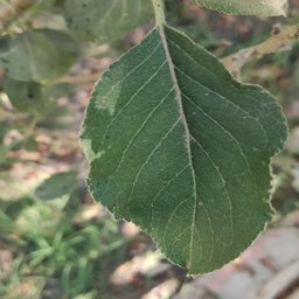
\includegraphics[width=2cm]{images/Introduction/EgyPLI/Xception/IMG_20240710_162039_original.png} \\[-1mm]
					\scriptsize Apple (EPLI)
				\end{tabular}
				&
				\begin{tabular}[c]{c}
					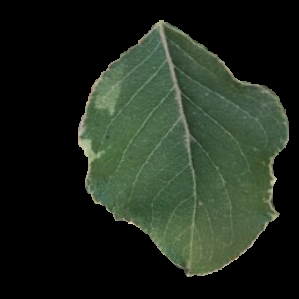
\includegraphics[width=2cm]{images/Introduction/EgyPLI/Xception/IMG_20240710_162039_segmented.png}
				\end{tabular}
				&
				\begin{tabular}[c]{c}
					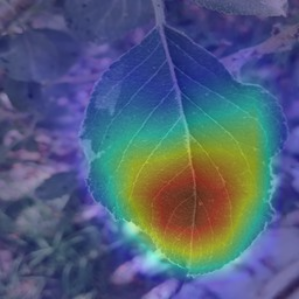
\includegraphics[width=2cm]{images/Introduction/EgyPLI/Xception/IMG_20240710_162039_clean.png} \\[-1mm]
					\scriptsize LMOS: 1.00
				\end{tabular}
				&
				\begin{tabular}[c]{c}
					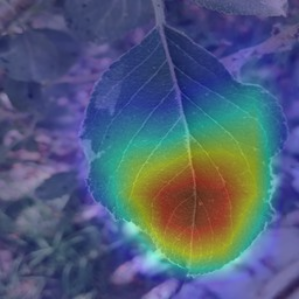
\includegraphics[width=2cm]{images/Introduction/EgyPLI/Xception/IMG_20240710_162039_hue.png} \\[-1mm]
					\scriptsize LMOS: 1.00
				\end{tabular}
				&
				\begin{tabular}[c]{c}
					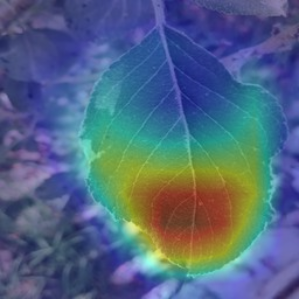
\includegraphics[width=2cm]{images/Introduction/EgyPLI/Xception/IMG_20240710_162039_blur.png} \\[-1mm]
					\scriptsize LMOS: 1.00
				\end{tabular}
				&
				\begin{tabular}[c]{c}
					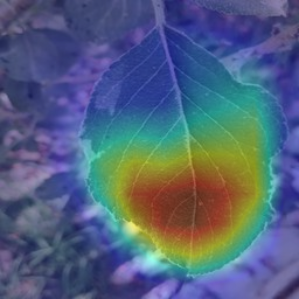
\includegraphics[width=2cm]{images/Introduction/EgyPLI/Xception/IMG_20240710_162039_contrast.png} \\[-1mm]
					\scriptsize LMOS: 1.00
				\end{tabular}
				&
				\begin{tabular}[c]{c}
					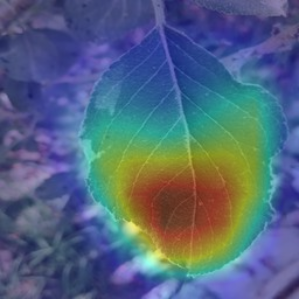
\includegraphics[width=2cm]{images/Introduction/EgyPLI/Xception/IMG_20240710_162039_compression.png} \\[-1mm]
					\scriptsize LMOS: 1.00
				\end{tabular}
				\\
				\midrule
				
				\begin{tabular}[c]{@{}l@{}}
					\textbf{Model:} Custom CNN \\
					\textbf{Accuracy:} 99.45\% \\
					\textbf{Mean LMOS:} 0.1900 \\
					\textbf{ETI:} 0.5922 \\
					\textbf{ERI:} 0.7944
				\end{tabular}
				&
				\begin{tabular}[c]{c}
					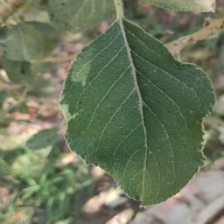
\includegraphics[width=2cm]{images/Introduction/EgyPLI/Custom_CNN/IMG_20240710_162039_original.png} \\[-1mm]
					\scriptsize Apple (EPLI)
				\end{tabular}
				&
				\begin{tabular}[c]{c}
					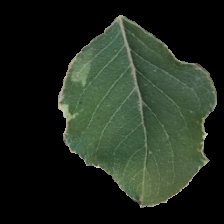
\includegraphics[width=2cm]{images/Introduction/EgyPLI/Custom_CNN/IMG_20240710_162039_segmented.png}
				\end{tabular}
				&
				\begin{tabular}[c]{c}
					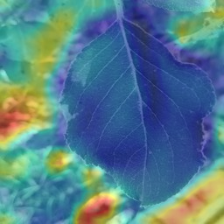
\includegraphics[width=2cm]{images/Introduction/EgyPLI/Custom_CNN/IMG_20240710_162039_clean.png} \\[-1mm]
					\scriptsize LMOS: 0.00
				\end{tabular}
				&
				\begin{tabular}[c]{c}
					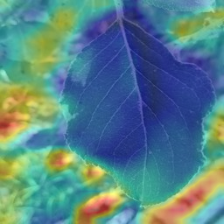
\includegraphics[width=2cm]{images/Introduction/EgyPLI/Custom_CNN/IMG_20240710_162039_hue.png} \\[-1mm]
					\scriptsize LMOS: 0.00
				\end{tabular}
				&
				\begin{tabular}[c]{c}
					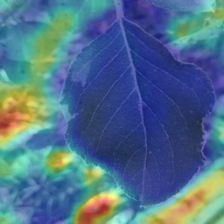
\includegraphics[width=2cm]{images/Introduction/EgyPLI/Custom_CNN/IMG_20240710_162039_blur.png} \\[-1mm]
					\scriptsize LMOS: 0.00
				\end{tabular}
				&
				\begin{tabular}[c]{c}
					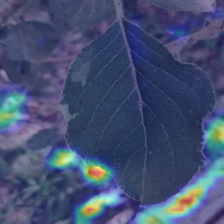
\includegraphics[width=2cm]{images/Introduction/EgyPLI/Custom_CNN/IMG_20240710_162039_contrast.png} \\[-1mm]
					\scriptsize LMOS: 0.00
				\end{tabular}
				&
				\begin{tabular}[c]{c}
					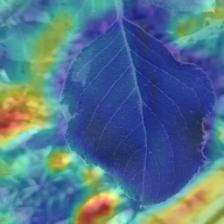
\includegraphics[width=2cm]{images/Introduction/EgyPLI/Custom_CNN/IMG_20240710_162039_compression.png} \\[-1mm]
					\scriptsize LMOS: 0.00
				\end{tabular}
				\\
				\midrule
				
				\begin{tabular}[c]{@{}l@{}}
					\textbf{Model:} Xception \\
					\textbf{Accuracy:} 95.05\% \\
					\textbf{Mean LMOS:} 0.7800 \\
					\textbf{ETI:} 0.8653 \\
					\textbf{ERI:} 0.8982
				\end{tabular}
				&
				\begin{tabular}[c]{c}
					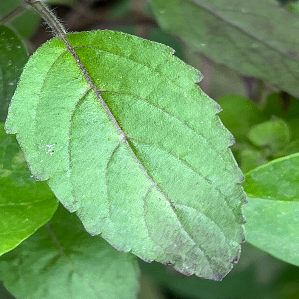
\includegraphics[width=2cm]{images/Introduction/BDML/Xception/IMG_9012_original.png} \\[-1mm]
					\scriptsize O. tenuiflorum (BDML)
				\end{tabular}
				&
				\begin{tabular}[c]{c}
					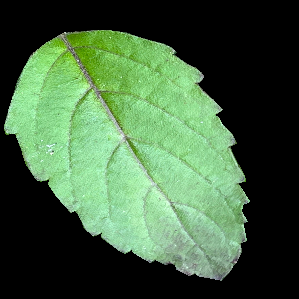
\includegraphics[width=2cm]{images/Introduction/BDML/Xception/IMG_9012_segmented.png}
				\end{tabular}
				&
				\begin{tabular}[c]{c}
					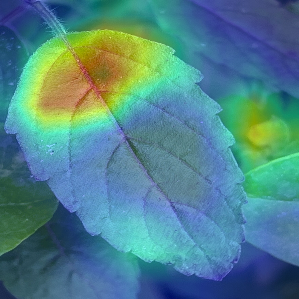
\includegraphics[width=2cm]{images/Introduction/BDML/Xception/IMG_9012_clean.png} \\[-1mm]
					\scriptsize LMOS: 1.00
				\end{tabular}
				&
				\begin{tabular}[c]{c}
					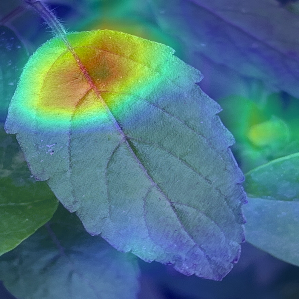
\includegraphics[width=2cm]{images/Introduction/BDML/Xception/IMG_9012_hue.png} \\[-1mm]
					\scriptsize LMOS: 1.00
				\end{tabular}
				&
				\begin{tabular}[c]{c}
					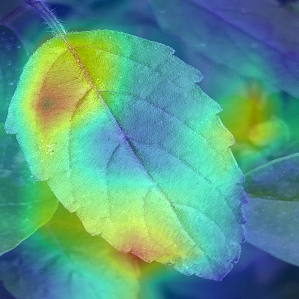
\includegraphics[width=2cm]{images/Introduction/BDML/Xception/IMG_9012_blur.png} \\[-1mm]
					\scriptsize LMOS: 0.903
				\end{tabular}
				&
				\begin{tabular}[c]{c}
					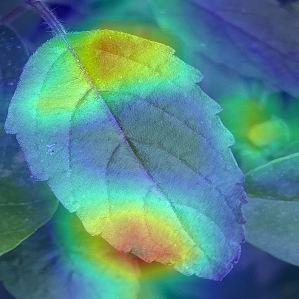
\includegraphics[width=2cm]{images/Introduction/BDML/Xception/IMG_9012_contrast.png} \\[-1mm]
					\scriptsize LMOS: 0.812
				\end{tabular}
				&
				\begin{tabular}[c]{c}
					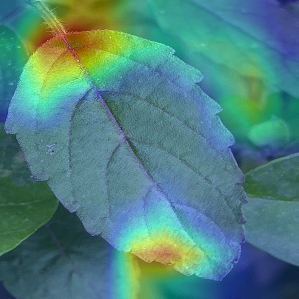
\includegraphics[width=2cm]{images/Introduction/BDML/Xception/IMG_9012_compression.png} \\[-1mm]
					\scriptsize LMOS: 0.785
				\end{tabular}
				\\
				\midrule
				
				\begin{tabular}[c]{@{}l@{}}
					\textbf{Model:} Inception V3 \\
					\textbf{Accuracy:} 93.07\% \\
					\textbf{Mean LMOS:} 0.3344 \\
					\textbf{ETI:} 0.6325 \\
					\textbf{ERI:} 0.7898
				\end{tabular}
				&
				\begin{tabular}[c]{c}
					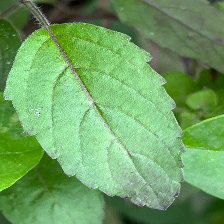
\includegraphics[width=2cm]{images/Introduction/BDML/Inception_V3/IMG_9012_original.png} \\[-1mm]
					\scriptsize O. tenuiflorum (BDML)
				\end{tabular}
				&
				\begin{tabular}[c]{c}
					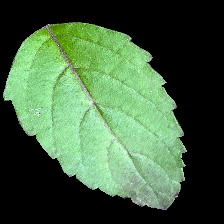
\includegraphics[width=2cm]{images/Introduction/BDML/Inception_V3/IMG_9012_segmented.png}
				\end{tabular}
				&
				\begin{tabular}[c]{c}
					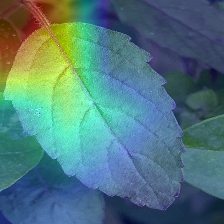
\includegraphics[width=2cm]{images/Introduction/BDML/Inception_V3/IMG_9012_clean.png} \\[-1mm]
					\scriptsize LMOS: 0.383
				\end{tabular}
				&
				\begin{tabular}[c]{c}
					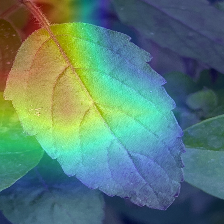
\includegraphics[width=2cm]{images/Introduction/BDML/Inception_V3/IMG_9012_hue.png} \\[-1mm]
					\scriptsize LMOS: 0.659
				\end{tabular}
				&
				\begin{tabular}[c]{c}
					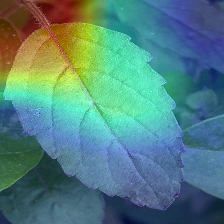
\includegraphics[width=2cm]{images/Introduction/BDML/Inception_V3/IMG_9012_blur.png} \\[-1mm]
					\scriptsize LMOS: 0.477
				\end{tabular}
				&
				\begin{tabular}[c]{c}
					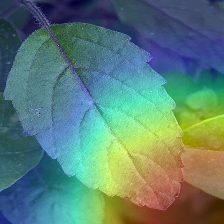
\includegraphics[width=2cm]{images/Introduction/BDML/Inception_V3/IMG_9012_contrast.png} \\[-1mm]
					\scriptsize LMOS: 0.390\textsuperscript{*}
				\end{tabular}
				&
				\begin{tabular}[c]{c}
					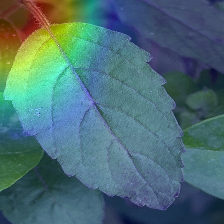
\includegraphics[width=2cm]{images/Introduction/BDML/Inception_V3/IMG_9012_compression.png} \\[-1mm]
					\scriptsize LMOS: 0.176
				\end{tabular}
				\\
				\bottomrule
			\end{tabular}%
		}
	\end{table*}
	
	% ==========================================
	% TABLE 2: Grad-CAM Visualization on Flower Datasets
	% ==========================================
	\begin{table*}[htbp]
		\centering
		\renewcommand{\arraystretch}{1.3}
		\caption{Grad-CAM visualization on Flower datasets (FLRS and FR).}
		\label{tab:model_robustness_flower}
		\resizebox{\textwidth}{!}{%
			\begin{tabular}{C{3.5cm} C{2.2cm} C{2.2cm} C{2.2cm} C{2.2cm} C{2.2cm} C{2.2cm} C{2.2cm}}
				\toprule
				\textbf{Model Metrics} & \textbf{Original} & \textbf{True Mask (M)} & \textbf{Clean} & \textbf{Hue} & \textbf{Blur} & \textbf{Contrast} & \textbf{Compression} \\
				\midrule
				
				\begin{tabular}[c]{@{}l@{}}
					\textbf{Model:} Xception \\
					\textbf{Accuracy:} 88.28\% \\
					\textbf{Mean LMOS:} 0.6869 \\
					\textbf{ETI:} 0.7849 \\
					\textbf{ERI:} 0.9308
				\end{tabular}
				&
				\begin{tabular}[c]{c}
					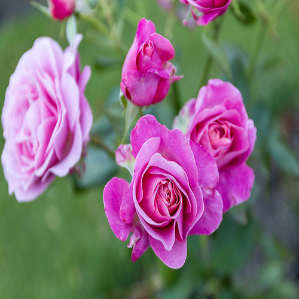
\includegraphics[width=2cm]{images/Introduction/tensorflow_dataset/Xception/11944957684_2cc806276e_original.png} \\[-1mm]
					\scriptsize Rose (FLRS)
				\end{tabular}
				&
				\begin{tabular}[c]{c}
					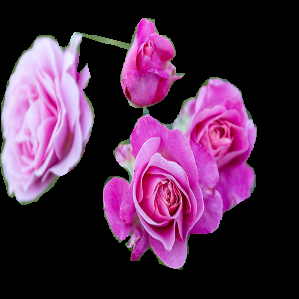
\includegraphics[width=2cm]{images/Introduction/tensorflow_dataset/Xception/11944957684_2cc806276e_segmented.png}
				\end{tabular}
				&
				\begin{tabular}[c]{c}
					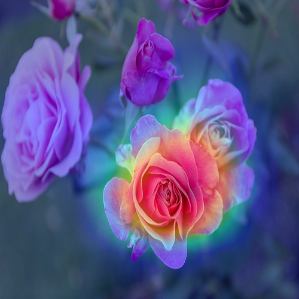
\includegraphics[width=2cm]{images/Introduction/tensorflow_dataset/Xception/11944957684_2cc806276e_clean.png} \\[-1mm]
					\scriptsize LMOS: 1.00
				\end{tabular}
				&
				\begin{tabular}[c]{c}
					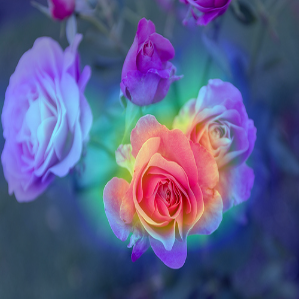
\includegraphics[width=2cm]{images/Introduction/tensorflow_dataset/Xception/11944957684_2cc806276e_hue.png} \\[-1mm]
					\scriptsize LMOS: 1.00
				\end{tabular}
				&
				\begin{tabular}[c]{c}
					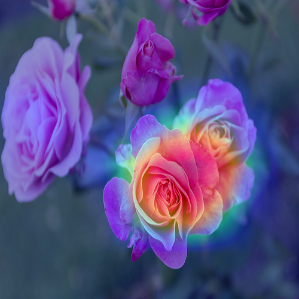
\includegraphics[width=2cm]{images/Introduction/tensorflow_dataset/Xception/11944957684_2cc806276e_blur.png} \\[-1mm]
					\scriptsize LMOS: 1.00
				\end{tabular}
				&
				\begin{tabular}[c]{c}
					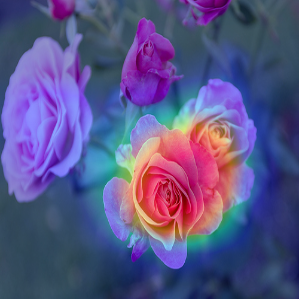
\includegraphics[width=2cm]{images/Introduction/tensorflow_dataset/Xception/11944957684_2cc806276e_contrast.png} \\[-1mm]
					\scriptsize LMOS: 1.00
				\end{tabular}
				&
				\begin{tabular}[c]{c}
					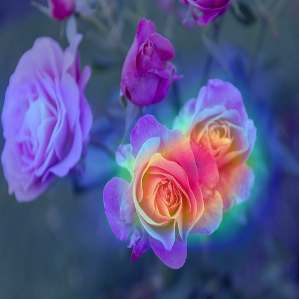
\includegraphics[width=2cm]{images/Introduction/tensorflow_dataset/Xception/11944957684_2cc806276e_compression.png} \\[-1mm]
					\scriptsize LMOS: 1.00
				\end{tabular}
				\\
				\midrule
				
				\begin{tabular}[c]{@{}l@{}}
					\textbf{Model:} Inception V3 \\
					\textbf{Accuracy:} 82.29\% \\
					\textbf{Mean LMOS:} 0.3749 \\
					\textbf{ETI:} 0.5989 \\
					\textbf{ERI:} 0.8593
				\end{tabular}
				&
				\begin{tabular}[c]{c}
					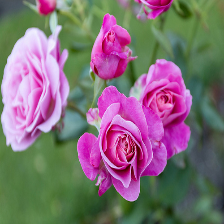
\includegraphics[width=2cm]{images/Introduction/tensorflow_dataset/Inception_V3/11944957684_2cc806276e_original.png} \\[-1mm]
					\scriptsize Rose (FLRS)
				\end{tabular}
				&
				\begin{tabular}[c]{c}
					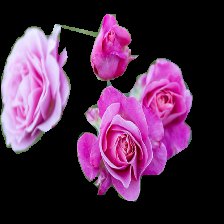
\includegraphics[width=2cm]{images/Introduction/tensorflow_dataset/Inception_V3/11944957684_2cc806276e_segmented.png}
				\end{tabular}
				&
				\begin{tabular}[c]{c}
					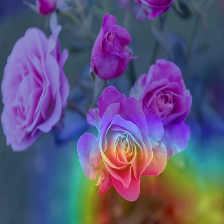
\includegraphics[width=2cm]{images/Introduction/tensorflow_dataset/Inception_V3/11944957684_2cc806276e_clean.png} \\[-1mm]
					\scriptsize LMOS: 0.305
				\end{tabular}
				&
				\begin{tabular}[c]{c}
					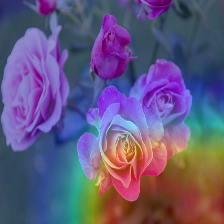
\includegraphics[width=2cm]{images/Introduction/tensorflow_dataset/Inception_V3/11944957684_2cc806276e_hue.png} \\[-1mm]
					\scriptsize LMOS: 0.219
				\end{tabular}
				&
				\begin{tabular}[c]{c}
					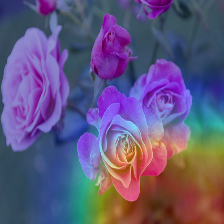
\includegraphics[width=2cm]{images/Introduction/tensorflow_dataset/Inception_V3/11944957684_2cc806276e_blur.png} \\[-1mm]
					\scriptsize LMOS: 0.181
				\end{tabular}
				&
				\begin{tabular}[c]{c}
					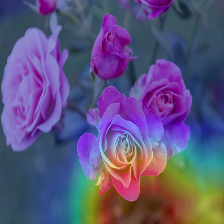
\includegraphics[width=2cm]{images/Introduction/tensorflow_dataset/Inception_V3/11944957684_2cc806276e_contrast.png} \\[-1mm]
					\scriptsize LMOS: 0.219
				\end{tabular}
				&
				\begin{tabular}[c]{c}
					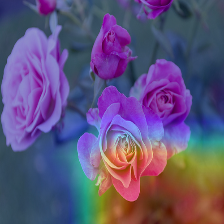
\includegraphics[width=2cm]{images/Introduction/tensorflow_dataset/Inception_V3/11944957684_2cc806276e_compression.png} \\[-1mm]
					\scriptsize LMOS: 0.214
				\end{tabular}
				\\
				\midrule
				
				\begin{tabular}[c]{@{}l@{}}
					\textbf{Model:} Xception \\
					\textbf{Accuracy:} 90.32\% \\
					\textbf{Mean LMOS:} 0.6029 \\
					\textbf{ETI:} 0.7531 \\
					\textbf{ERI:} 0.9689
				\end{tabular}
				&
				\begin{tabular}[c]{c}
					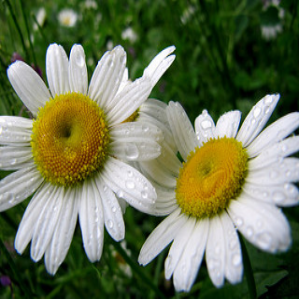
\includegraphics[width=2cm]{images/Introduction/FR/Xception/4668543441_79040ca329_n_original.png} \\[-1mm]
					\scriptsize Daisy (FR)
				\end{tabular}
				&
				\begin{tabular}[c]{c}
					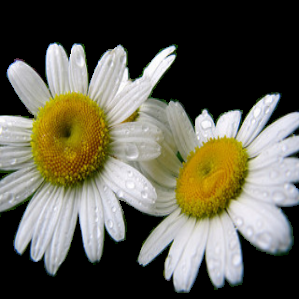
\includegraphics[width=2cm]{images/Introduction/FR/Xception/4668543441_79040ca329_n_segmented.png}
				\end{tabular}
				&
				\begin{tabular}[c]{c}
					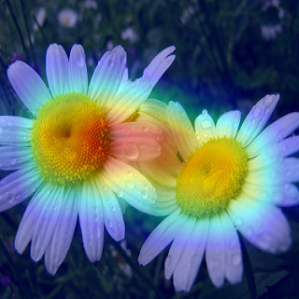
\includegraphics[width=2cm]{images/Introduction/FR/Xception/4668543441_79040ca329_n_clean.png} \\[-1mm]
					\scriptsize LMOS: 1.00
				\end{tabular}
				&
				\begin{tabular}[c]{c}
					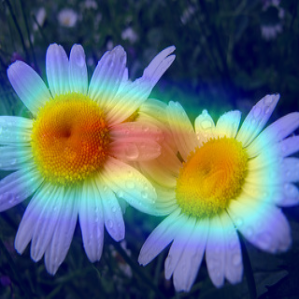
\includegraphics[width=2cm]{images/Introduction/FR/Xception/4668543441_79040ca329_n_hue.png} \\[-1mm]
					\scriptsize LMOS: 1.00
				\end{tabular}
				&
				\begin{tabular}[c]{c}
					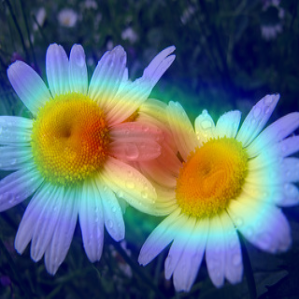
\includegraphics[width=2cm]{images/Introduction/FR/Xception/4668543441_79040ca329_n_blur.png} \\[-1mm]
					\scriptsize LMOS: 1.00
				\end{tabular}
				&
				\begin{tabular}[c]{c}
					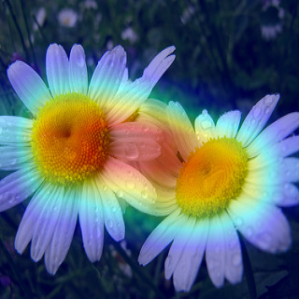
\includegraphics[width=2cm]{images/Introduction/FR/Xception/4668543441_79040ca329_n_contrast.png} \\[-1mm]
					\scriptsize LMOS: 1.00
				\end{tabular}
				&
				\begin{tabular}[c]{c}
					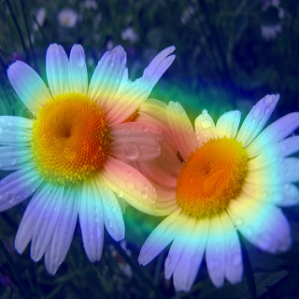
\includegraphics[width=2cm]{images/Introduction/FR/Xception/4668543441_79040ca329_n_compression.png} \\[-1mm]
					\scriptsize LMOS: 1.00
				\end{tabular}
				\\
				\midrule
				
				\begin{tabular}[c]{@{}l@{}}
					\textbf{Model:} Inception V3 \\
					\textbf{Accuracy:} 88.25\% \\
					\textbf{Mean LMOS:} 0.3063 \\
					\textbf{ETI:} 0.5944 \\
					\textbf{ERI:} 0.8827
				\end{tabular}
				&
				\begin{tabular}[c]{c}
					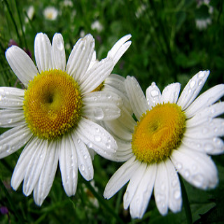
\includegraphics[width=2cm]{images/Introduction/FR/Inception_V3/4668543441_79040ca329_n_original.png} \\[-1mm]
					\scriptsize Daisy (FR)
				\end{tabular}
				&
				\begin{tabular}[c]{c}
					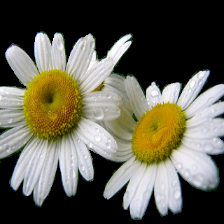
\includegraphics[width=2cm]{images/Introduction/FR/Inception_V3/4668543441_79040ca329_n_segmented.png}
				\end{tabular}
				&
				\begin{tabular}[c]{c}
					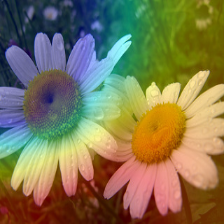
\includegraphics[width=2cm]{images/Introduction/FR/Inception_V3/4668543441_79040ca329_n_clean.png} \\[-1mm]
					\scriptsize LMOS: 0.633
				\end{tabular}
				&
				\begin{tabular}[c]{c}
					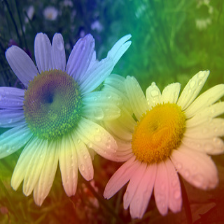
\includegraphics[width=2cm]{images/Introduction/FR/Inception_V3/4668543441_79040ca329_n_hue.png} \\[-1mm]
					\scriptsize LMOS: 0.583
				\end{tabular}
				&
				\begin{tabular}[c]{c}
					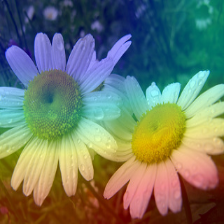
\includegraphics[width=2cm]{images/Introduction/FR/Inception_V3/4668543441_79040ca329_n_blur.png} \\[-1mm]
					\scriptsize LMOS: 0.550
				\end{tabular}
				&
				\begin{tabular}[c]{c}
					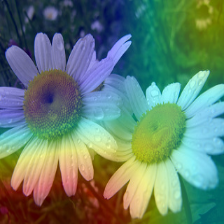
\includegraphics[width=2cm]{images/Introduction/FR/Inception_V3/4668543441_79040ca329_n_contrast.png} \\[-1mm]
					\scriptsize LMOS: 0.388
				\end{tabular}
				&
				\begin{tabular}[c]{c}
					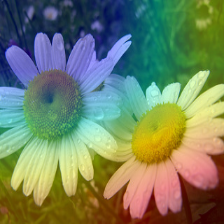
\includegraphics[width=2cm]{images/Introduction/FR/Inception_V3/4668543441_79040ca329_n_compression.png} \\[-1mm]
					\scriptsize LMOS: 0.505
				\end{tabular}
				\\
				\bottomrule
			\end{tabular}%
		}
	\end{table*}
